\graphicspath{{Chapters/Chapter_isat-predict/}}

\chapter{Optimizing mirror configurations in the LAPD using machine learning}
\label{ch:opt_ML}

\begin{abstract}
\todo{Shorten; less detail}
Modern machine learning (ML) techniques based on neural networks (NNs) provide an opportunity to learn trends directly from data, which is the first step towards automating fusion science. The goal of this work is to demonstrate that ML-based insight extraction is possible and useful. The Large Plasma Device (LAPD) is a remarkably flexible basic plasma science device with a high shot rep rate (0.25-1 Hz) and relatively reproducible plasmas. The LAPD also capable of high-spatial-resolution measurements, such as the ion saturation current ($I_\text{sat}$ — proportional to density and the square root of electron temperature). These traits of the LAPD make it the ideal machine for producing datasets for experimenting with ML techniques. Time-averaged ion saturation current data were recorded from randomly sampled machine configurations in the LAPD in order to create a minimally biased, relatively diverse dataset. Over 100,000 shots in over 45 different machine configurations were collected. Magnetic field strengths, fueling parameters, and the discharge voltage were varied in these experiments. A five-model, 200k parameter NN ensemble was trained on this dataset using a negative log-likelihood (NLL) loss function. This ensemble and loss formulation enable the breakdown of uncertainty into aleatoric and epistemic components. During inference, these NNs can be evaluated quickly (~4 million predictions per second on an RTX 3090). This fast inference enables creation of a comprehensive set of $I_\text{sat}$ values (over 127 million) in any LAPD machine configuration at any position bounded by the training set. Trends inferred using this method, such as effects on $I_\text{sat}$ of introducing mirrors or changing the discharge current, are consistent with intuition. In addition, these predictions can be used to optimize LAPD behavior. The required machine conditions for minimizing or maximizing axial variation (quantified by the standard deviation of on-axis $I_\text{sat}$ values) can be found via comprehensive search over the predicted $I_\text{sat}$ values. The corresponding machine conditions were then executed on the LAPD. The optimized, experimental axial $I_\text{sat}$ profiles yielded similar behavior to model predictions, but with appreciable absolute error. This error could be caused by the lack of absolute calibration of the Langmuir probes. The predicted uncertainty provides a relative metric for gauging model confidence. Ultimately, ML techniques provide a new way of extracting insight from experiments. LAPD plasmas can be optimized by using simple and straightforward neural networks, which is a first in the magnetized plasma (or fusion) community. All code and data used in this study will be made freely available.

\end{abstract}

%\pacs{}% insert suggested PACS numbers in braces on next line

%\maketitle %\maketitle must follow title, authors, abstract and \pacs

\section{Introduction}

Machine learning (ML) techniques, particularly the use of neural networks (NNs), have become increasingly used in magnetized confinement fusion research to control and stabilize fusion plasmas. Plasma devices are complicated systems with many possible settings, actuators, and actuator states. From an ML point of view, these parameters are a high-dimensional input into a system whose output (plasma behavior) we wish to understand. Because this space is high-dimensional, understanding how these devices work is often time-consuming and requires careful planning. We seek to accelerate understanding of fusion devices with the goal of putting fusion on the grid as fast as possible.  

Many studies have used ML for profile prediction on a variety of tokamaks, particularly for real-time prediction and control. A model was built to predict several quantities, such as electron density and temperature, in DIII-D using NNs\cite{abbate_data-driven_2021}. A reservoir computing approach was also performed\cite{jalalvand_real-time_2022} featuring the ability to quickly adapt to new situations or other tokamaks. Entire shots have also been auto-regressively predicted using Recurrent NNs (RNNs)\cite{char_full_2024}. RNNs have also been used for autoregressive predictions on the EAST\cite{wan_east_2022} and KSTAR tokamaks\cite{seo_feedforward_2021,seo_development_2022}, the latter of which were used to train a reinforcement learning-based controller. Electron temperature profiles have also been predicted using dense NNs on the J-TEXT tokamak \cite{dong_machine_2021}.

Much focus in the fusion community has been on instability mitigation in tokamaks, particularly the catastrophic loss of plasma confinement know as a disruption. The tearing instability is a common cause of disruptions in tokamaks, and the mitigation of these instabilities has been performed in DIII-D using reinforcement learning\cite{seo_avoiding_2024}. In general, there has been much work on predicting disruptions, the most important of them being an RNN approach by Kates-Harbeck et al.\cite{kates-harbeck_predicting_2019} and the random forest approach taken by Rea et al.\cite{rea_real-time_2019}. A good overview of pre-2022 disruption prediction activity can be found in Vega et al.\cite{vega_disruption_2022}. 

The process of inferring trends using data-driven methods has been relatively uncommon. Finding scaling laws are one such task that is at the extreme high-bias end of these data-driven methods. Nonetheless, ML techniques have been used as a tool to discover scaling laws. Classical ML techniques were used to find the boundary between safe and disruptive operational space on the JET tokamak\cite{murari_investigating_2020}. Genetic programming was then used to find a symbolic, power-law expression for this boundary to provide interpretability. Similarly, the development of the new Maris density limit\cite{maris_correlation_2024} used ML techniques -- neural networks, random forests, linear SVMs, and linear regressions -- to find a stability boundary by treating the fit as a classification problem. The power law derived from the linear SVM far outperforms that traditional Greenwald scalings when validated across many tokamaks. This new scaling also predicts, in advance, the density limit violation within a discharge much better than the Greenwald or other scalings. 

The laser plasma research field (ICF, wakefield, and others) has used machine learning extensively for different applications, enumerated in the review by Dopp et al. \cite{dopp_data-driven_2023}. We have not been able to find the extra step of using ML methods to infer trends in plasma research in general. Data-driven plasma science in general has been reviewed by Anirudh et al. \cite{anirudh_2022_2023}.

This study takes these data-driven methods a step further: instead of learning a model for particular task (e.g., disruption prediction or profile prediction), we scan along inputs of this model to infer trends. Trend inference applied in this way is new to magnetized plasma research. 

The goal of this study is to develop a data-driven model that can provide insight into how machine settings impact the plasmas produced in the Large Plasma Device (LAPD) in lieu of a theoretical model. We demonstrate the capability to infer trends in a particular diagnostic signal, the time-averaged ion saturation current ($I_\text{sat}$) for any mirror (or anti-mirror) field geometry in a variety of machine configurations. Trends of the effect of a varying a particular machine setting can be predicted in a data-efficient manner by training on many randomly-selected machine settings. This partially randomized data acquisition is a first for magnetized plasma research. Additionally, to the authors' best knowledge, this is the first time NNs have been used to directly infer trends in magnetized plasmas. Using this model, LAPD plasmas can also be optimized given any cost function, which we demonstrated by minimizing axial $I_\text{sat}$ variation. This global optimization is only possible using ML techniques. This work demonstrates the usefulness of a pure ML approach to modeling device operation and shows how this model can be exploited. We encourage existing ML projects and experiments to consider this approach if possible, but it may require assuming some risk to acquire diverse datasets.

This paper is organized as follows: section \ref{sec:data} discusses the LAPD and the data acquisition process. Development of the model and uncertainty quantification are discussed in sections \ref{sec:model_dev} and \ref{sec:uncertainty}, respectively. Validation of the predictions made by the model are shown in section \ref{sec:validation}. Inferring trends in discharge voltage and gas puff duration are presented in section \ref{sec:trends}. Optimizing the axial $I_\text{sat}$ profile is performed and validating the optimization on the LAPD can be seen in section \ref{sec:optimization}. The discussion, outlook, future work, and conclusions are discussed in sections \ref{sec:discussion} and \ref{sec:conclusion}.

\section{Data collection and processing}
\label{sec:data}

\subsection{The Large Plasma Device (LAPD)}

%\begin{enumerate}
%	\item LAPD diagram and coordinate system; diagnostics locations
%\end{enumerate}

The Large Plasma Device (LAPD)\cite{gekelman_upgraded_2016,qian_design_2023} is a basic plasma experiment located at the University of California, Los Angeles. The LAPD produces an up to 18m long, 1m diameter plasma column with densities up to $3 \times 10^{13}$ cm$^{-3}$ and temperatures up to 20 eV, though typical operation yields temperatures around 5 eV. Every 32 cm, the LAPD has unique ball valves between the solenoid coils that permit 3d movement of inserted probes. These probes enable the collection of time series data with high spatial resolution at virtually any point in the plasma column. The LAPD also has a discharge repetition rate, configurable between 0.25 and 1 Hz. Additionally, the LAPD has 13 independently controllable magnet power supplies to shape the geometry of the magnetic field along the length of the device. The discharge is formed by 38 cm diameter lanthanum hexaboride (LaB6) cathode\cite{qian_design_2023} and 72 cm molybdenum anode 0.5m (-z direction) at the southern end (+z) of the device. A cartoon of the LAPD and relevant coordinate system can be seen in fig. \ref{fig:LAPD_coords}. 

\begin{figure*}
	\centering
	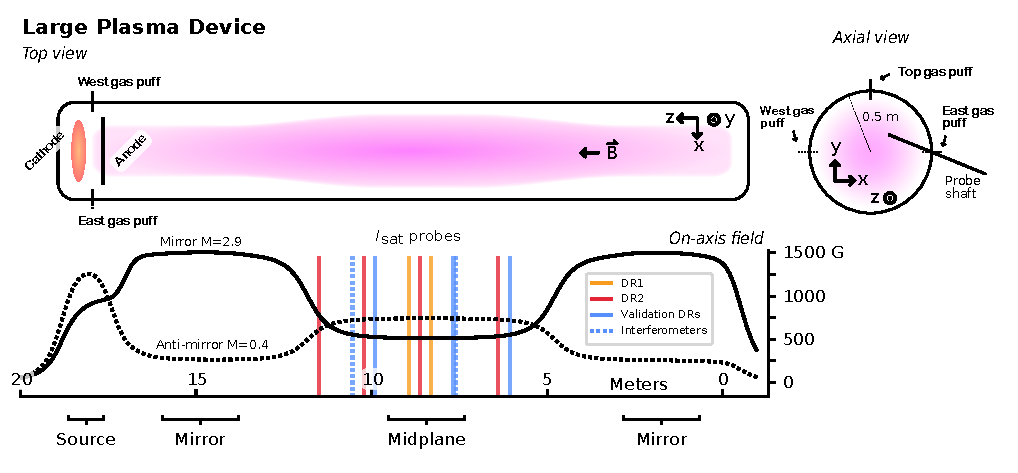
\includegraphics[width=\textwidth]{figures/LAPD+coordinates.pdf}
	\caption[size=12]{\label{fig:LAPD_coords}A cartoon of the Large Plasma Device, the coordinate system used, examples of a mirror and anti-mirror magnetic field configuration, and probe locations used in this study. The source, mirror, and midplane regions are labeled; the three fields were programmed independently.}
\end{figure*}

The LAPD has many actuators available for various physics studies. Components such as biasing rings, antennas, and an additional cathode, can be inserted into the LAPD. However, in this work we focus on the settings fundamental to the operation of the main cathode. In particular, the region half way between the cathode and anode contains three gas puff valves: East, West, and top. The opening size, duration, and triggering of these valves has a large impact on plasma formation. There is also a static gas fill system but it is not used in this study. The cathode-anode voltage (and more broadly, discharge power) also has a significant effect on the plasma density and temperature downstream of the source. The magnetic field configuration also greatly affects the plasmas produced. One main actuator not considered in this study is the cathode temperature because it takes many hours to adjust and equilibrate, limiting the diversity of any dataset collected.

This diagnostic coverage, high repetition rate, and high degree of configurability makes the LAPD a natural fit machine learning studies. 

\subsection{Data collection and processing of $I_\text{sat}$ signals}

Ion saturation current, referred to as $I_\text{sat}$, is measurement using a sufficiently negatively biased Langmuir probe such that only ions are collect. The measurement is proportional to $S n_e \sqrt{T_e}$, where S is the effective area of the probe. Since the area varies depending on the particular probe used for the measurement, the $I_\text{sat}$ displayed will be normalized to area. An $I_\text{sat}$ value of 1 mA/mm$^2$ corresponds to $n_e \approx 1\text{-}2\times 10^{12}$ cm$^{-3}$ for a $T_e$ from 4 to 1 eV.

Data were taken over two separate weeks, 14 months apart. The first run set will be referred to as \texttt{DR1} and the second as \texttt{DR2}. These run sets are further broken down into \em dataruns \em which are a collection of shots with the same machine conditions. 67 dataruns were collected in total. 

$I_\text{sat}$ signals were averaged from 10 to 20 ms. This range was chosen to avoid effects of ramp up and to average-out plasma fluctuations. Plasma profile evolution is not covered to limit the scope and compute required for this study. 
%An example plot of three $I_\text{sat}$ time series near x=y=0 can be seen in fig. \ref{fig:PP1_time-series-example} \todo{remove plot}. 
Note that the $I_\text{sat}$ time traces can vary significantly between axial (z) position and dataruns (read: machine settings). For the $I_\text{sat}$ signal on the same probe as a Langmuir sweep (\texttt{DR2} port 26, z=863 cm), the $I_\text{sat}$ signal was averaged only where the sweep was off (plus an additional 40 $\mu$s buffer) and not affecting the measurement. Some $I_\text{sat}$ signals in \texttt{DR1} saturated either the isolation amplifier or the digitizer and were removed from the dataset.

The machine parameters varied were the source field, mirror field, midplane field, gas puff valve voltage, gas puff duration, and discharge voltage. The source, mirror, and midplane regions are labeled in fig. \ref{fig:LAPD_coords}. The magnetic field in each of these regions effectively control the width of the plasma in those regions relative to the cathode. The gas puff voltage controls the rate of gas flow into the chamber while the valve is open. The relationship between gas puff voltage and this rate is not yet quantified. The gas puff duration is how long this voltage is applied to the gas puff piezo valve. The discharge voltage is the voltage the capacitor bank is charged to, which is then applied across the anode and cathode 10 ms after the gas puff voltage is applied. The discharge voltage is related to the discharge current (and thus total discharge power), but the current cannot be set ahead of time: it is determined by other machine settings.

These machine parameters -- with the exception of gas puff duration -- were randomly sampled via Latin-hypercube sampling (LHS) for 44 of the dataruns. Data were then collected with these settings. Gas puff duration was reduced for the last seven runs to 20, 10, or 5 ms. The breakdown of each setting in the dataset can be seen appendix \ref{sec:app_bias}, table \ref{tab:data_frac}. The top gas puff valve was used for only the first nine dataruns of \texttt{DR2} because of equipment issues.

Data were collected on the probes at equally spaced locations on a y=0 line (51 dataruns total) or an x-y grid (16 dataruns total). The spacing varied between 1.5 to 2 cm depending on the particular datarun and grid configuration. The axial positions of the probes were left fixed at six different locations in total. 895 cm and 831 for \texttt{DR1} and 1150, 1022, 863, and 639 cm for \texttt{DR2} (also shown in fig. \ref{fig:LAPD_coords}). 

Six shots were recorded per position with the exception of the first four dataruns in \texttt{DR1} with five shots. Note that each position may have some variation in the $I_\text{sat}$ value recorded, but the model will only learn the expected value. Generative models -- future work -- can instead directly learn the distribution.

%\begin{figure}
%	\centering
%	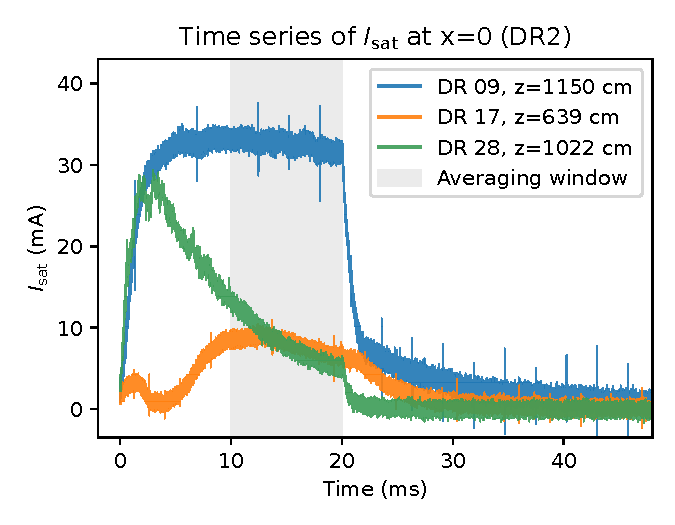
\includegraphics[width=\textwidth]{figures/PP1_time-series-example.pdf}
%	\caption[size=12]{\label{fig:PP1_time-series-example}Illustrative $I_\text{sat}$ traces from a Langmuir probe from \texttt{DR2} dataruns 09, 17, and 28 at ports 17, 33, and 21, respectively. Shot 1 of 6 shown. The signal is averaged over the filled region.}
%\end{figure}

%\begin{figure}
%	\centering
%	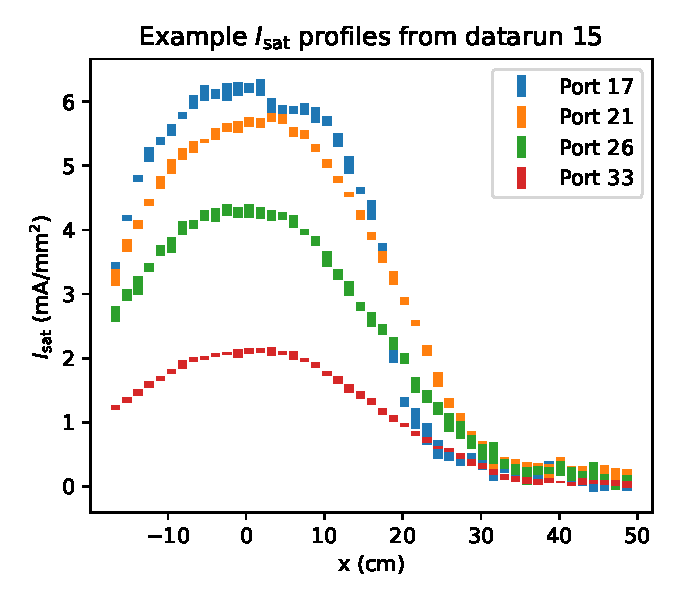
\includegraphics[width=\textwidth]{figures/PP1_isat_example_bars.pdf}
%	\caption[size=12]{\label{fig:PP1_isat_example}Examples of $I_\text{sat}$ profiles from \texttt{DR2} run 15. The bars represent the minimum and maximum of the six $I_\text{sat}$ measurements taken at that position. }
%\end{figure}
%
%\begin{figure}
%	\centering
%	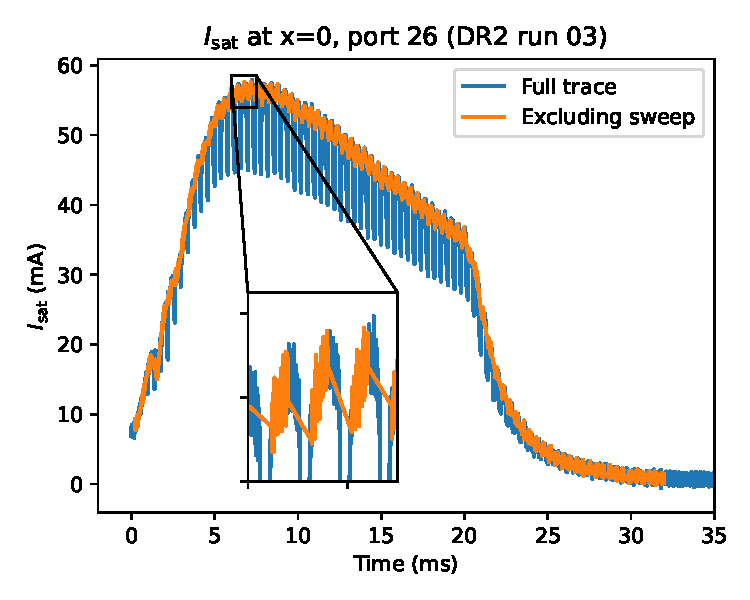
\includegraphics[width=\textwidth]{figures/PP1_isat_swept_probe.pdf}
%	\caption[size=12]{\label{fig:PP1_swept_probe}$I_\text{sat}$ traces from the swept probe (port 26) from \texttt{DR2} datarun 03, shot 1 of 6. The orange curve is excluding times when a sweep is active on an opposing tip. }
%\end{figure}

\subsection{Dataset distribution and bias}

Planar data were typically recorded overnight, leading to many more shots for that particular machine state. In general, $\approx 64\%$ of the shots recorded were planes. 

Only seven dataruns with gas puff durations less than 38 ms were recorded. These dataruns were taken as an attempt to see mirror-related interchange instabilities in higher-temperature, less collisional regimes. Because of the small amount of dataruns in non-random machine configurations the training data is heavily biased towards the 38 ms gas puff duration. Good model performance on regimes similar to these short gas-puff runs is not expected.

The top gas puff valve was also used for the first nine runs of \texttt{DR2}.

The $I_\text{sat}$ distribution is dissimilar between \texttt{DR1} and \texttt{DR2}. \texttt{DR1} appears to have a more uniform distribution than \texttt{DR2} does. Combining the two datasets results in many $I_\text{sat}$ examples near 0 mA/mm$^2$ and a sharp decrease in number of examples above 10 mA/mm$^2$. We expect or model to be biased towards fitting lower $I_\text{sat}$ values better, and to perform badly in cases with very high $I_\text{sat}$ values. Data bias is further discussed in appendix \ref{sec:app_bias}.

The final input size for the neural networks is 12: source field, mirror field, midplane field, gas puff voltage, discharge voltage, gas puff duration, three positions (x, y, z), probe rotation, run set flag, and the top gas puff flag. The last two were added as the project continued. The data are scaled to the peak-to-peak for each input; there are no outliers in the dataset so all scaled values are sane.

%\begin{enumerate}
%	\item $I_\text{sat}$ distribution (done)
%\end{enumerate}

%\begin{figure}
%	\centering
%	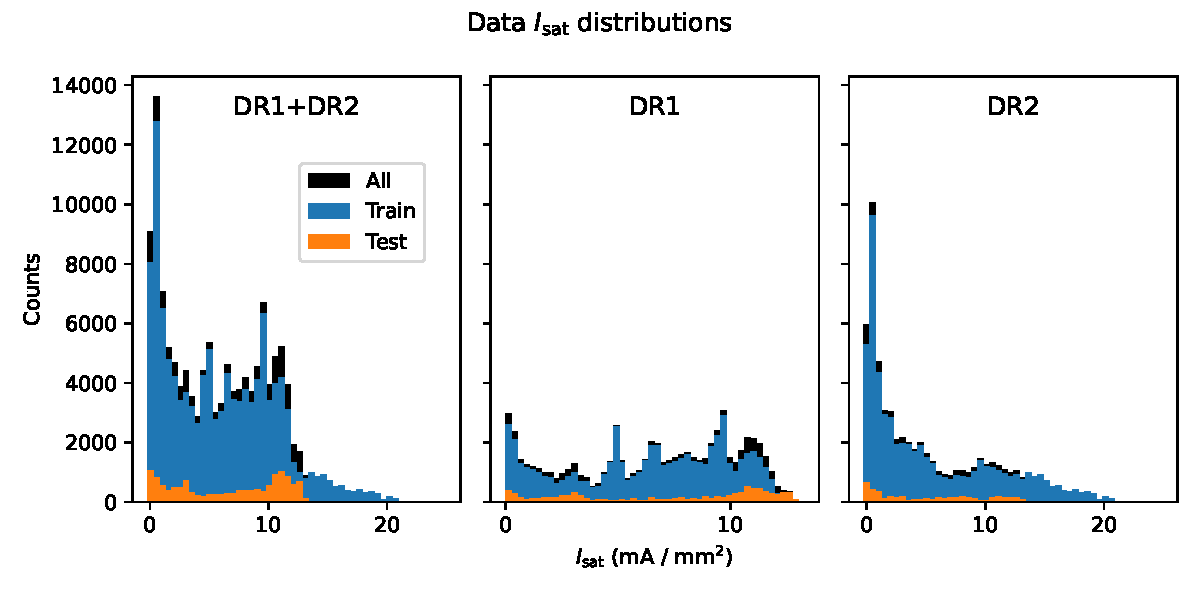
\includegraphics[width=\textwidth]{figures/PP1_02_isat_distribution.pdf}
%	\caption[size=12]{\label{fig:PP1_02_isat_distribution}Distribution of $I_\text{sat}$ signals. \texttt{DR1} appears to have a more uniform distribution than \texttt{DR2} does. Combining the two datasets results in many $I_\text{sat}$ examples near 0 mA/mm$^2$ and a sharp decrease in number of examples above 10 mA/mm$^2$. From these histograms we expect or model to be biased towards fitting lower $I_\text{sat}$ values better, and to perform badly in cases with very high $I_\text{sat}$ values.}
%\end{figure}

\section{Model development, training}
\label{sec:model_dev}

\subsection{Initial training details}

The loss used to train the model was simply the mean-squared error (MSE): 
\begin{equation}
	\mathcal{L}_\text{MSE}=\frac{1}{m}\sum_{i=1}^m \left(f\left(x_i\right) - y_i \right)^2
\end{equation} 
where $x_i$ is the inputs for the $i$th example, $y_i$ is the ground truth, $m$ is the number of examples in a given batch, and $f$ is the neural network. During training, overfitting was tracked using a traditional 80-20 train-validation random split. Unless stated otherwise, a dense neural network, 4 layers deep and 512 units wide, was trained with AdamW using a learning rate of $3\times10^{-4}$. Leaky ReLU activations were used instead of tanh to avoid vanishing gradients and adaptive gradient clipping \cite{seetharaman_autoclip_2020} (cutting gradients norms above the 90th percentile of recent norms) was used to mitigate exploding gradients.


\subsection{Baselines for mean-squared error}

A summary of the performance of all models can be seen in table \ref{tab:loss_summary}.

A model was first trained with zeroed-out inputs as a baseline and to validate the data pipeline. This model effectively has only a single, learnable bias parameter at the input. This process yields a validation loss (simply MSE in this case) of 0.036. 

%A model was also overfit on 8 examples and a single batch (128 examples) to verify that the training process operating correctly. 

A simple dense model (4 layers, 512 wide with one output; 794113 parameters, tanh activations) was trained on a zeroed-out input as a baseline for determining that the model is learning anything at all. This process yields a validation loss of 0.036. A linear model obviously cannot fit the dataset because profiles, amongst other features are never linear. However, a simple linear model can provide a performance baseline to help spot bugs when training more complex models. This baseline linear reaches a training and validation loss (MSE) of around 0.014.

\begin{table}
	\small
	\centering
	\caption{Summary of test set losses for different training data and ensembles}
	\label{tab:loss_summary}
	\begin{tabular}{l l l}
		Model & MSE $\times 10^{-3}$ \\
		\hline
		Zeroed-input & 36 \\
		Linear model & 14 \\
		Linear with tanh & 11 \\
		\hline
		9 dataruns & 7.0\\
		19 dataruns & 6.9 \\
		29 dataruns & 4.2 \\
		39 dataruns & 4.1 \\ 
		49 dataruns & 3.4 \\
		\texttt{DR1} only & $6.4$ \\
		\texttt{DR2} only & $5.4$ \\
		Full set, large model & $2.8$ \\
		Full set average & $3.6 \pm 0.56$ \\
		Full set ensemble & $2.9 \pm 1.1$ \\
		\hline
%		``Run set" flag average & $2.1 \pm 0.15$ \\
		``Run set" flag ensemble & $1.9 \pm 0.64$ \\
		``Top gas puff" flag & 1.8 \\
		
	\end{tabular}
\end{table}

\subsection{Effects of reducing the training set}

Several models were trained with dataruns cut out, decreasing the diversity of the training set. The test set was kept fixed. Loss on the test set monotonically increases with decreasing diversity. 

An equal amount of dataruns from each run set were randomly and iteratively removed from the training set. Results when changing training set diversity are roughly what was anticipated: model performance on the test set decreased with the decrease in diversity. 

Multiple models with different seeds were trained for the full-training-set model to measure the performance variance over model parameters. The \texttt{DR1}-only dataset was evaluated on the \texttt{DR1}-only test set, and likewise with \texttt{DR2}. The cross-run test set losses were incredibly high, near or above the zero-input baseline of $3.6 \times 10^{-2}$. The ``best" model was a large 12-deep 2048-wide dense network trained on the full training dataset, evaluated at 30 epochs. Longer training or larger models may yield better test set results, but will likely not come close to the training and validation losses which are on the order of $10^{-5}$. 

One unexpected result is that models trained on a single run set appear to perform worse when evaluated on the test set (from that particular run set) compared to the mixed training set of the same size (green arrows vs blue x). This fact indicates that mixing dataruns, despite different probe calibrations and cathode state, provides beneficial information on the structure of the $I_\text{sat}$ measurement. This model is able to leverage information in both dataruns despite potential differences in the effect of the machine settings and the cathode condition.

%Skepticism is warranted, however, because the variance over model parameters may be able to account for most, if not all, of the performance difference as suggested by the full-set ensemble. The variance caused by random datarun selection may also account for some of the difference; this variance was not measured and could be considerable. The effect of varying the training and test datasets will be discussed in section \ref{subsec:cross-validation}.

\subsection{Improving performance with machine state flags}

Run sets \texttt{DR1} and \texttt{DR2} were taken roughly 14 months apart so the machine state was different from the two runs. In \texttt{DR1}, only one turbo pump was operating leading to much higher neutral pressures than in the \texttt{DR2} run set. A new flag (mean-centered and scaled) was added to the inputs indicating which run set each shot belongs to. All the predictions in this work use the \texttt{DR2} run set flag (a value of 1.0) because turning off the turbopumps is not a commonly desired mode of operating the LAPD. The inclusion of this flag also provides the model the ability to distinguish between the probe calibration differences between \texttt{DR1} and \texttt{DR2}. An ensemble prediction with this run set flag brings the test set MSE down to $1.9 \times 10^{-3}$.  

A flag indicating when the top gas puff valve was enabled in \texttt{DR2} was also added to all training data, allowing the model to further distinguish between different fueling cases. The addition of this flag incrementally improved test set MSE to $1.8 \times 10^{-3}$ and so remains as the input.

%\begin{enumerate}
%	\item Baseline models plot (done)
%	\item Losses vs dataset diversity (done)
%\end{enumerate}

%\begin{figure}
%	\centering
%	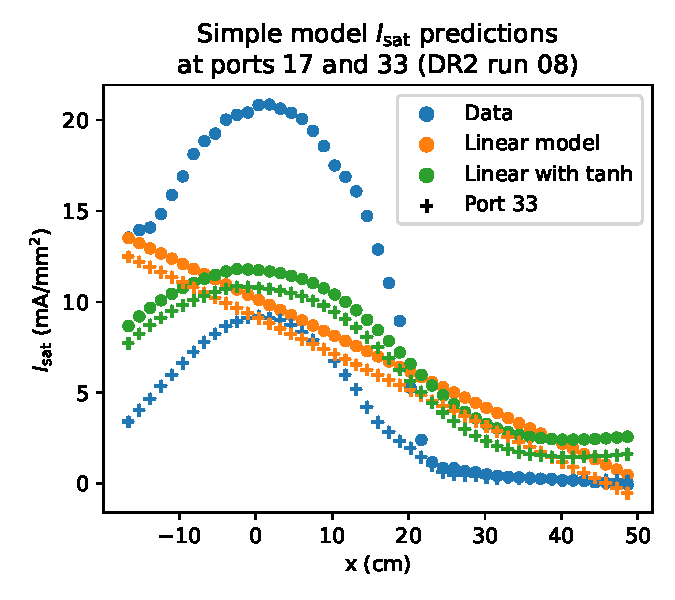
\includegraphics[width=\textwidth]{figures/PP1_linear_simple_vs_data.pdf}
%	\caption[size=12]{\label{fig:PP1_linear_simple_data}$I_\text{sat}$ profiles and predictions for ports 17 and 33 based on inputs from \texttt{DR2} run 08 using a liner and linear-with-tanh models. \texttt{DR2} run 08 is in the training set. The ``data" points are averaged over six shots. Run 08 was chosen for its representative performance; ports 17 and 33 were chosen to demonstrate the maximal axial variation (across 511 cm). These models fail to describe the data accurately.}
%\end{figure}
 
%\begin{figure}
%	\centering
%	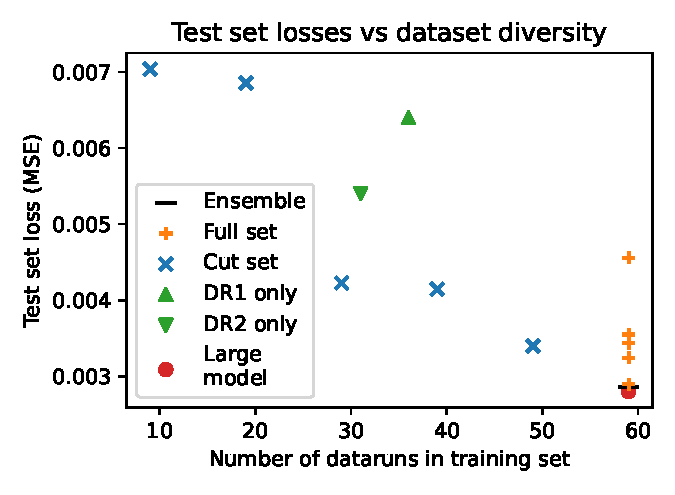
\includegraphics[width=\textwidth]{figures/PP1_test-loss_vs_dataset.pdf}
%	\caption[size=12]{\label{fig:PP1_validation_diversity}Several models were trained with dataruns cut out, decreasing the diversity of the training set. The test set was kept fixed. Loss on the test set monotonically increases with decreasing diversity. }
%\end{figure} 

\section{Uncertainty quantification}
\label{sec:uncertainty}

\subsection{$\beta$-NLL loss and learning rate scheduling}

One can interpolate between an MSE loss and Guassian NLL loss by introducing an adaptive scaling factor $\text{StopGrad}(\sigma_i^{2\beta})$ into the NLL loss function (eq. \ref{eq:loss_beta-NLL}):

\begin{equation}
	\mathcal{L}_{\beta-\text{NLL}} = \frac{1}{2}\left( \log{\sigma^2_i(\mathbf{x}_n)} +\frac{\left(\mu_i(\mathbf{x}_n) - y_n\right)^2}{\sigma^2_i (\mathbf{x}_n)} \right) \text{StopGrad}\left(\sigma_i^{2\beta}\right)
	\label{eq:loss_beta-NLL}
\end{equation}

for example $n$ and model $i$, with an implicit expectation over training examples. $\beta=0$ yields the original Gaussian NLL loss function and $\beta=1$ yields the MSE loss function, so introducing a $\beta$ factor can be interpreted as interpolating between these two loss functions. Thus, this factor improves MSE performance by scaling via an effective learning rate for each example (which is why StopGrad is used) \cite{seitzer_pitfalls_2022}, and may also improve both aleatoric and epistemic uncertainty quantification \cite{valdenegro-toro_deeper_2022}. $\beta=0.5$ was used by default in this study. This $\beta$-NLL loss function also improved training stability.

This typical negative-log likliehood loss assumes the prediction -- the likelihood of $y$ given input $\mathbf{x}$: $p(y|\mathbf{x})$ -- follows a Gaussian distribution. Treating each prediction as an independent random variable (considering each model in the ensemble is sampled from some weight distribution $\theta \sim p(\theta | \mathbf{x}, y)$) and finding the mean of the random variables yields a normal distribution with mean $\mu_* (\mathbf{x}) = \langle \mu_i(\mathbf{x}) \rangle $ and variance $\sigma^2_* = \langle \sigma^2_i(\mathbf{x}) + \mu^2_i(\mathbf{x}) \rangle - \mu^2_* (\mathbf{x})$ where $\langle \rangle$ indicates an average over the ensemble.

The ensemble predictive uncertainty can be broken down into the aleatoric and epistemic components \cite{valdenegro-toro_deeper_2022}: the aleatoric uncertainty is $\langle \sigma^2_i (\mathbf{x}) \rangle$ and the epistemic uncertainty is $\langle \mu^2_i (\mathbf{x}) \rangle - \mu^2_* (\mathbf{x}) = \text{Var}\lbrack\mu_i (\mathbf{x}) \rbrack$. The intuition behind these uncertainties is that the random fluctuations in the recorded data are captured in the variance of a single network, $\sigma^2_i$, so the average of these variances represents that sort of randomness present. If the choice of model were to make a significant difference, we'd expect the predicted mean for a single model, $\mu_i$, to fluctuate quite a bit, which is captured by $\text{Var}\lbrack\mu_i (\mathbf{x}) \rbrack$. 

%Using the $\beta$-NLL loss, the model is slightly better calibrated, but barely worth discussing. 

Modifying the learning rate over time (also known as scheduling) is known to improve model learning. A few schedules were tried: constant learning rate ($\gamma = 3 \times 10^{-4}$), $\gamma \propto \text{epoch}^{-1}$, $\gamma \propto \exp{(\text{epoch})}$, and $\gamma \propto \text{epoch}^{-1/2}$. The epoch is the training step divided by the number of batches in one epoch, so ``epoch" in this case takes on a floating-point value. $\gamma \propto \text{epoch}^{-1}$ appears to give the best test set loss by a test MSE of $1 \times 10^{-4}$, and any schedule beats a constant learning rate by $2-4 \times 10^{-4}$. 
%The differences in test set losses are small, but the difference in training and validation losses are quite significant, with the constant learning rate loss being three times higher. 

%\begin{enumerate}
%	\item Cross validation plot (done)
%	\item z-score histogram (done)
%	\item Calibration via weight decay scan (done)
%	\item Profiles with different weight decays (done)
%\end{enumerate}

\subsection{Cross-validation MSE}

Multiple train-test set pairs were created. Test set 0 is the hand-picked dataset, chosen to contain a diverse set of machine settings and probe movements. The other six were randomly compiled without replacement while keeping the number of dataruns from \texttt{DR1} and \texttt{DR2} equal. Seven model ensembles (35 NNs total) were trained to evaluate the effect of test set choice on perceived model performance. The median ensemble test set MSE for these seven sets was $2.13 \times 10^{-3}$ with a mean of $3.6 \times 10^{-3}$. The handpicked dataset had an ensemble test set MSE of $1.85 \times 10^{-3}$, indicating that the choice of dataruns was adequately representative because the MSE is close to the median cross-validated value. This median MSE will be used to estimate model prediction error in addition to uncertainty quantification. This cross-validation also provides an error estimate if the models were to be trained on \emph{all} dataruns. It was also seen that ensembles always out-perform the average single-model prediction.

%The median of the cross-validation ensemble performance for the test set is roughly the same as the MSE for testing set 0, so our choice of dataruns for the testing set appears reasonable. The calibration of the model also varies across dataruns, which can be investigated. Ideally, knowing the models train well and having an idea of the cross-validated error, it should be possible to train on all data in it's entirety and still have some reasonable estimate of the error of the model.

%\begin{figure}
%	\centering
%	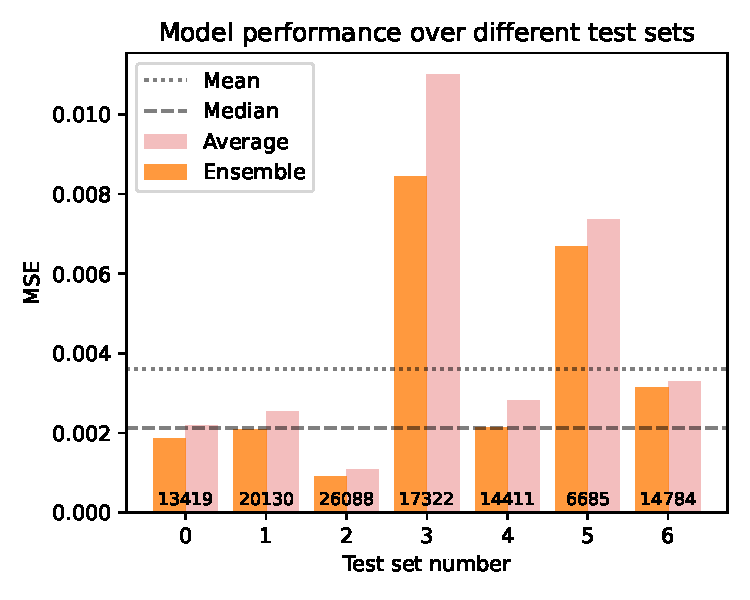
\includegraphics[width=\textwidth]{figures/cv-beta-NLL-valid-mse.pdf}
%	\caption[size=12]{\label{fig:cv-beta-NLL-valid-mse}Model performance as measured by MSE over test sets with different dataruns. Test set 0 is the hand-picked dataset, and the rest were randomly compiled without replacement (though separate for \texttt{DR1} and \texttt{DR2}). The number at the bottom of the bar chart is the number of shots in the testing set. The median test set performance is very close to the hand picked (set 0) performance. Ensembles always out-perform the average single-model prediction.}
%\end{figure}

\subsection{Model calibration via weight decay}

An attempt is made to calibrate the model uncertainty. The predicted uncertainty may not provide a suitable predicted $I_\text{sat}$ range when compared to the measured value. Calibrating the model means changing the predicted uncertainty range so that the real, measured values fall within that range according to some distribution, such as a Gaussian in this case. One of the ways assessing this calibration is by the z-score of predictions, where $z_n=x_n - \mu_n / \sigma_n(x_n)$ for example $x_n$, predicted mean $\mu_n$, and standard deviation $\sigma_n$. Perfect model calibration would mean an identical z-score distribution $\mathcal{N}(\mu=0, \sigma=1)$ for the training a test sets. When evaluated on the training set, the training set z-score distribution is consistent with this Gaussian distribution. The standard deviation of this z-score distribution should be 1.

Increased weight decay can lead to better model calibration \cite{guo_calibration_2017}. Many ensembles were trained to determine the best weight decay coefficient between 0 and 50, determined by the distribution of z-scores of the training and test examples, seen in fig. \ref{fig:beta-NLL_wd_model_performance}. Increasing the weight decay increases the test MSE and decreases its z-score standard deviation. This large standard deviation is caused by outliers. Excluding z-scores magnitudes above 10, or 4.4\% of the test set, yields a standard deviation of 2.53. Nonetheless, the trend remains that increasing weight decay leads to smaller test set z-score standard deviations. However, the test set MSE increases after a weight decay of 1. This increase in test MSE means that the model is making less accurate predictions, but the model is better calibrated. Highly biased models are better calibrated, but come at great expense of mean prediction error. At the weight decay value of 50, the model has worse error than a linear model. Despite the attempts using weight decay, the model never becomes well-calibrated: the predicted uncertainty is always too low by a factor of 2 to 5. 

%As seen in fig. \ref{fig:extrapolation-variance_wd-comparison}, the uncertainty predictions are not useful except for models with low weight decays.
 
%A comparison of many different weight decay coefficients can be seen in fig. \ref{fig:weight_decay-model}; 20 was determined to be a good weight decay value. The ``knee" value of 30 was not chosen because the distribution of z-scores looked odd. The training and test z-score distribution can be seen in fig. \ref{fig:weight_decay-distribution}. Note that weight decay (coefficient $\lambda$) is implemented in \texttt{AdamW} as $\theta_t = \theta_{t-1} -\gamma\lambda \ \theta_{t-1}$ so learning would be impossible above the reciprocal of the learning rate of $\gamma = 3 \times 10^{-4}$.

%Despite a well-calibrated test set error, the predictions on the training and test sets are not very good. An MSE of $\approx 3 \times 10^{-3}$ may sound decent (RMSE of $\approx 5\%$) but the error is weighted by the low $I_\text{sat}$ values at the edge of the plasma (see fig. \ref{fig:PP1_02_isat_distribution}) which are relatively easy to predict correctly. 

%\begin{figure}
%	\centering
%	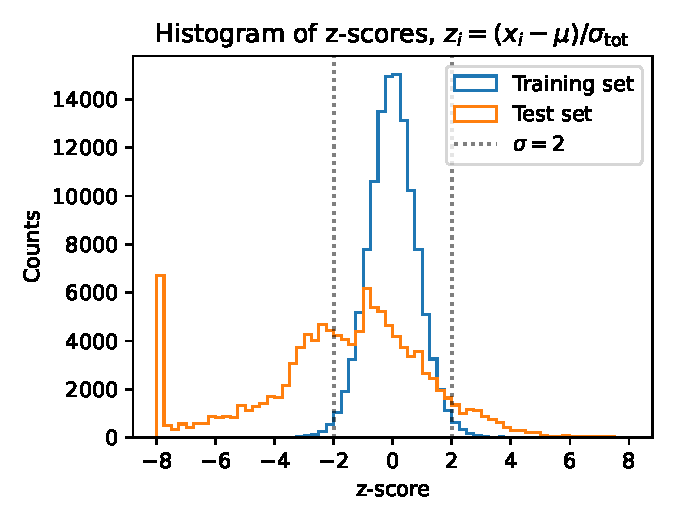
\includegraphics[width=\textwidth]{figures/z-score_wd-0_paperplot.pdf}
%	\caption[size=12]{\label{fig:z-score_wd-0_paperplot}Z-scores for the training and testing set for the model with a weight decay coefficient of zero. The magnitude of counts for the test set is scaled up by a factor of 8.8 (the train-to-test example ratio). The histograms are clipped between -8 and 8 with a bin width of 0.25; the spike at the negative sisse of the test set histogram is from a long tail.}
%\end{figure}
%
\begin{figure}
	\centering
	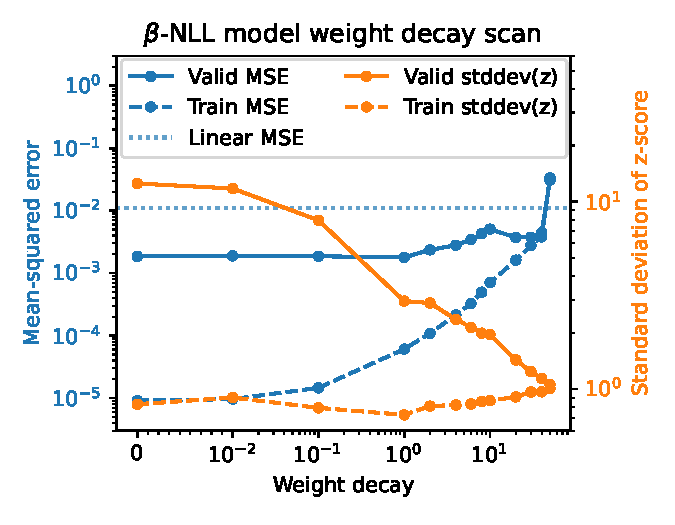
\includegraphics[width=\textwidth]{figures/beta-NLL_wd_model_performance.pdf}
	\caption[size=12]{\label{fig:beta-NLL_wd_model_performance}Model performance and calibration for different weight decays. Highly biased models are better calibrated, but come at great expense of mean prediction error. At the weight decay value of 50, the model has worse error than a linear model. Note the linear scale below $10^{-2}$.}
\end{figure}

Despite the better calibration, the uncertainty predicted by the model is decidedly worse: the uncertainty is similar across an entire profile, and when projected beyond the training data, the total uncertainty remains largely constant. See fig. \ref{fig:extrapolation-profile-var_two}. On the other hand, the zero weight decay model exhibits relatively increasing uncertainty beyond the bounds of the training data. Although not well-calibrated, this uncertainty can provide a hint of where the model lacks confidence relative to other predictions, even though the uncertainty is much less than it should be.

\begin{figure*}
	\centering
	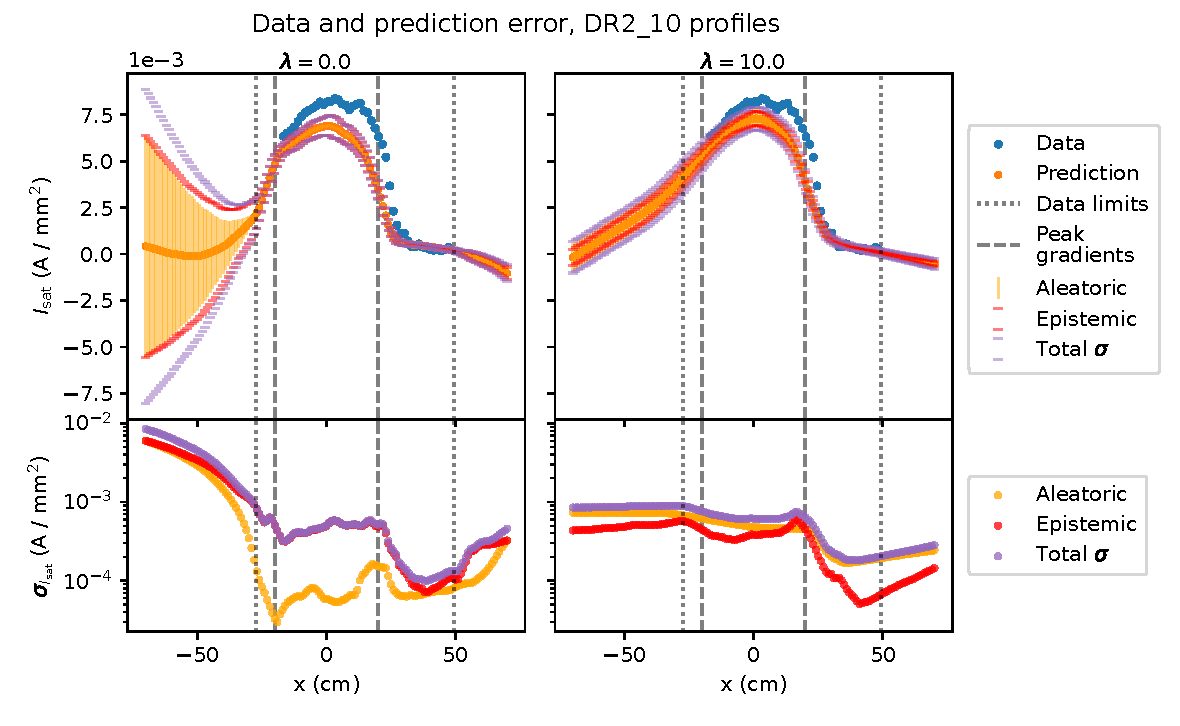
\includegraphics[width=360pt]{figures/extrapolation-profile-variance_DR2_10_wd-comparison_two.pdf}
	\caption[size=12]{\label{fig:extrapolation-profile-var_two}Model extrapolation performance (top plots) with uncertainty (bottom plots) for a model ensemble trained on a $\beta$-NLL loss function. \texttt{DR2} run 10 was chosen as an illustrative example. The \em relative \em uncertainty appears to be more useful when zero weight decay ($\lambda = 0$, left) is used: the uncertainty increases when the model is predicting outside its training data along the x-axis.}
\end{figure*}

\section{Evaluating model performance}
\label{sec:validation}

Model performance is evaluated in three ways by comparing against intuition from geometry, an absolute measurement, and extrapolated machine conditions. 

%\begin{enumerate}
%	\item Geometrical changes with changing mirrors (done)
%	\item Single shot prediction (done)
%	\item Extrapolation plot comparison (done)
%\end{enumerate}

\subsection{Checking geometrical intuition}

From geometric arguments (and experience), we know that modifying the mirror geometry can control the effective width of the plasma. One way to check that the machine model is learning appropriate trends is to check with this intuition. Namely, when the magnetic field at the source is not equal to the field at the probe, the probe will see the plasma expanded (or contracted) by roughly a factor of $\sqrt{B_\text{probe}/B_{source}}$. The cathode is about 35 cm in diameter, so a magnetic field ratio of 3 would give produce a plasma approximately 60 cm in diameter. All the probes used in this study are in or very close to the zero-curvature region of a mirror.

\todo{the end of this section doesn't match the plot.}
To check this intuition, the model is given the following inputs: $B_\text{source}$=500 G, $B_\text{mirror}$=1500 G, $B_\text{midplane}$=500 G, discharge voltage=110 V, gas puff voltage=70 V, gas puff duration=38 ms, run set flag=\texttt{DR2} and top gas puff=off. The discharge voltage and gas puffing parameters were arbitrarily chosen. The x coordinate is scanned from 0 to 30 cm, and the z coordinate from 640 to 1140 cm. This discharge is then modified by separately changing $B_\text{source}$ to 1500 G and $B_\text{midplane}$ to 750 G (M=1.5). %and $B_\text{mirror}$ to 750 G. 
The x profiles at the midplane (z=790 cm) of the reference M=3 prediction, source field change, and midplane field change, all scaled to cathode radius, can be seen in fig. \ref{fig:changing-B-field_M=3_x-prof}. Changing the source field to 1500 G increases the $I_\text{sat}$ towards the edge of the plasma, as expected. When the midplane field is increased, the $I_\text{sat}$ values decrease at the edge and increase at the core (x=0 cm), which implies a thinner plasma column and is consistent with previously measured behavior. When only the mirror field is modified, the strongest effect on $I_\text{sat}$ is on or near x=0 cm, and the plasma column width does not appear to appreciably change. Strong axial $I_\text{sat}$ gradients are present in these predicted discharges.

\begin{figure}
	\centering
	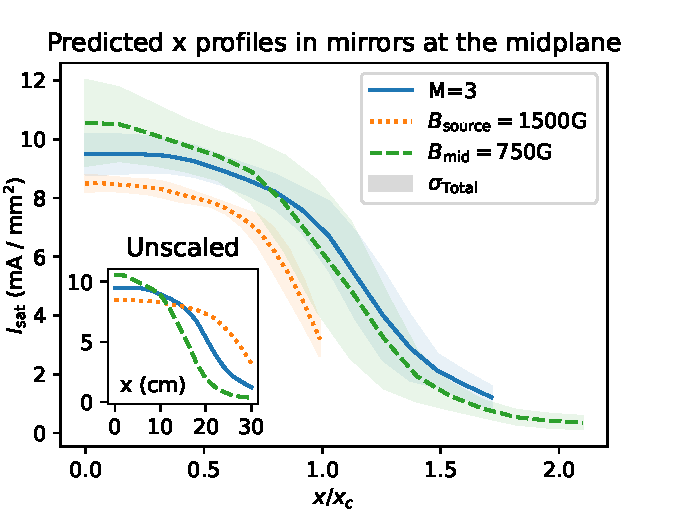
\includegraphics[width=\textwidth]{figures/changing-B-field_M=3_x-prof.pdf}
	\caption[size=12]{\label{fig:changing-B-field_M=3_x-prof}Plot of various mirror configurations scaled to the cathode radius $x_c=17.5$ cm at the midplane (z=790 cm). When scaled according to the expected magnetic expansion, the profiles generally agree. The smaller the plasma diameter (and thus smaller volume), the higher the peak in $I_\text{sat}$ at the core, as expected. }
\end{figure}

\subsection{Directly comparing prediction to measurement}

%Data were collected on September 18th, 2024 to validate the predictions made for the strongest axial variation. Given the model inputs were incorrect (the gas puff voltage was swapped with discharge voltage), this optimization is broadly wrong. However, because the prescribed gas puff voltage and discharge voltage were the same (90 V) and within the bounds of the actuator training data, we can still use these data for validation. 

$I_\text{sat}$ measurements were taken with the following LAPD machine settings: $B_\text{source}$=1250 G, $B_\text{mirror}$=500 G, $B_\text{midplane}$=1500 G, discharge voltage=90 V, gas puff voltage=90 V, gas puff duration=38 ms, run set flag=\texttt{DR2} and top gas puff=off. These settings were from a previous discharge optimization attempt. The probes utilized were the permanently-mounted 45$^\circ$ probe drives. These probes were known to have identical effective areas relative to each other from the previous experiment and from analyzing the discharge rampup.

Because of data acquisition issues, only a single useful shot was collected at a nominal -45$^\circ$ angle 10 cm past the center (x=0 cm, y=0 cm) of the plasma on three probes at z-positions of 990, 767, and 607 cm (ports 22, 29, and 34, respectively). The probe drives were slightly uncentered, leading to the real coordinates of the probes to be around x $=9.75$ cm and y $=-8.4$ cm. Note that the model can predict anywhere in LAPD bounded by the training data, so off-axis measurements are not an issue.
%These probes were also not centered so the positions were slightly further +x and -y. Issues (scripts crashing) with the probe drives and oscilloscope readout resulted in only a single shot being recorded. 
The resulting predictions using these coordinates and machine conditions can be seen in fig. \ref{fig:strongest_axial_var-validation}. 
%The off-axis predictions and $I_\text{sat}$ measurements result in less-smooth profile when compared with the on-axis prediction. 
The model reproduces the axial trend well, but slightly underestimates $I_\text{sat}$ on an absolute comparison. However, given the lack of absolute $I_\text{sat}$ calibration for both this validation datarun and the training data, the agreement of the absolute $I_\text{sat}$ values may be coincidental. Additionally, the cathode appeared to be in a low-emissivity state that is, at the moment, not well understood. Nevertheless, the axial trends match. 

\begin{figure}
	\centering
	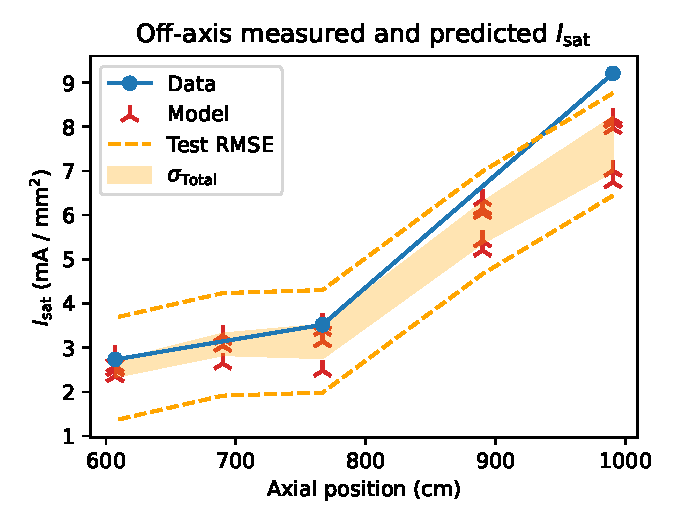
\includegraphics[width=\textwidth]{figures/strongest_axial_var-validation.pdf}
	\caption[size=12]{\label{fig:strongest_axial_var-validation}Data collected at off-axis positions around x $=9.75$ cm and y $=-8.4$ cm are compared with predictions from the machine learning model at the same points in addition to two interpolating predictions. The model predicts the trend well, but underestimates $I_\text{sat}$ in general. The shaded orange region is the total model uncertainty ($\sigma = \sqrt{\text{Var}}$).}
\end{figure}

An additional validation datarun was performed. For this run, the discharge voltage was increased to 160 V, and the source field changed to 822 G. The training data contains discharge voltages up to 150 V, so this case tests the extrapolation capabilities of the model. The comparison of model predictions and the measured data can be seen in fig. \ref{fig:measured-vs-predicted_160V}. As stated earlier, the absolute uncertainty provided of the model is not calibrated. However, note that the level of uncertainty provided by the model, as well as the large spread in model predictions, are much greater than seen in the interpolation regime (fig. \ref{fig:strongest_axial_var-validation}) and eclipses the cross-validated test set RMSE. We conclude that this model has good interpolation capabilities, but extrapolation -- as with any model -- remains difficult.

%Probe tip rotation was not accounted for in the prediction, but including the correct rotation produces uncertainty meeting or exceeding the test RMSE threshold because rotations at this angle have not been seen by the model. This probe tip rotation bias suggests that for this model probe rotation need not be correct for accurate predictions. The model performs worse when azimuthal symmetry is assumed by treating x as the radial coordinate and calculating the distance from x=y=0 cm. This degraded inference performance, also seen when training the model (section \ref{subsec:azimuthal_symmetry}) suggests that there is some intrinsic azimuthal asymmetry in the plasma, possibly caused by the horizontal gas puff injection near the source.

\begin{figure}
	\centering
	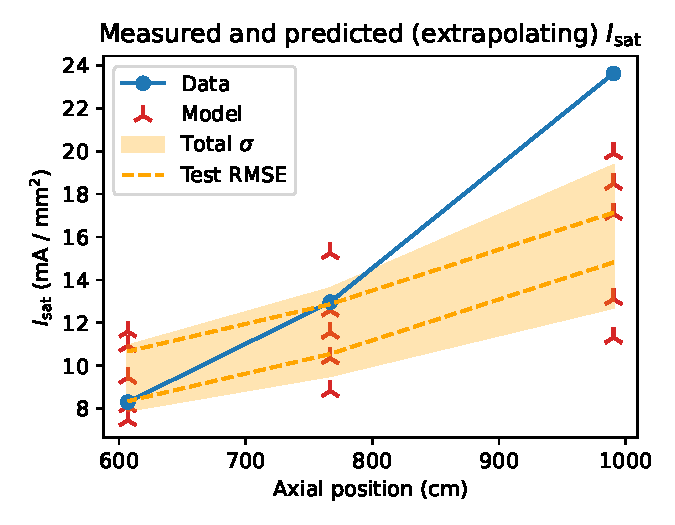
\includegraphics[width=\textwidth]{figures/measured-vs-predicted_160V.pdf}
	\caption[size=12]{\label{fig:measured-vs-predicted_160V}Measured vs predicted $I_\text{sat}$ values for an odd machine configuration with $B_\text{source}$=822 G and discharge voltage=160 V. The training data only covers discharge voltages up to 150 V The machine was also in an odd discharge state, so it's no surprise that the predicted uncertainty bounds are very large (even greater than the test set RMSE value) and that accuracy suffers.}
\end{figure}

\section{Inferring trends}
\label{sec:trends}

%\begin{enumerate}
%	\item Discharge voltage trends (done)
%	\item Discharge voltage trends -- real data
%	\item Axial gradient vs gas puff (done)
%\end{enumerate}

A systematic study of the impact of discharge voltages on $I_\text{sat}$ profiles has not been performed. Collecting both z- and x-axis profiles over a wide range of discharge voltages would take a considerable amount of time, mostly from the requirement to dismount and reattach the probes and probe drives along the length of the LAPD. We perform this study in silico using the learned model. Model input parameters were chosen to be common, reasonable values: 1 kG flat field, 80 V gas puff, 38 ms gas puff duration, run set=\texttt{DR2}, and top gas puff off. The 38 ms puff is used in these predictions because it is the most common gas puff duration in the training set, so the model is biased in favor of this gas puff setting. The results of changing the discharge voltage only can be seen in fig \ref{fig:discharge_voltage_effect}. Notably, the $I_\text{sat}$ increases across both axes. Steeper axial gradients are seen with lower discharge voltages, but peaked x-profiles are seen at higher discharge voltages. The area closer to the source region (+z direction) appears to have a steep drop but flatter profiles down the length of the machine. 

 Unfortunately the discharge current was not included as an output in the training set. Otherwise the effect of changes in discharge power, rather than simply voltage, could be computed. The discharge current -- and thus discharge power -- is set by cathode condition, cathode heater settings, and the downstream machine configuration, and thus cannot be set to a desired value easily before the discharge. Discharge voltage, however, can remain fixed.

\begin{figure}
	\centering
	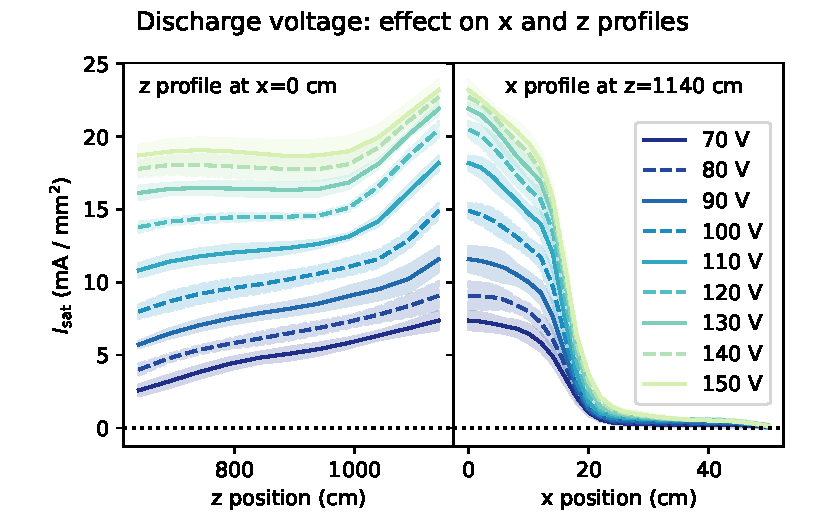
\includegraphics[width=\textwidth]{figures/discharge_voltage_effect.pdf}
	\caption[size=12]{\label{fig:discharge_voltage_effect}The z profile at x=0 cm and x profile at z=1140 cm for different discharge voltages. The $I_\text{sat}$ decreases with increasing voltage, and the error (filled regions) stays roughly the same, but in general increase slightly towards the cathode and at higher discharge voltages.}
\end{figure}

\todo{get plot from Shreekrishna?}

Of particular interest for some LAPD users is achieving the flattest possible axial profile. We explore this problem in the context of mirrors. The gas puff duration is known to be a large actuator for controlling density and temperature and so is explored as a way of shaping the axial profile. We predict discharges with a flat 1 kG field with the probe in the center. The discharge voltage was set at 110 (a reasonable, middle value) with the run set flag=\texttt{DR2} and top gas puffing=off. The inferred effect of gas puff duration on the axial gradient and axial gradient scale length can be seen in fig. \ref{fig:axial-grad_gas-puff.pdf}. Care was taken to handle the aleatoric (independent) uncertainty separately from the axially-dependent epistemic uncertainty. As seen in the figure, the mean axial gradient decreases when the gas puff duration is shortened. The gradient scale length also increases, so the mean gradient is not decreasing simply because the bulk $I_\text{sat}$ is decreasing. This result suggests that the gas puff duration may be a useful actuator to consider when planning future experiments. 

These applicability of these results are somewhat muted because the gas puff duration was not chosen randomly in the training discharges. Only 6 runs in the training set had gas puff durations less than 38 ms. Three were 5 ms, three were 10 ms, with each having mirror ratios 1, 3, and 6 and otherwise identical configurations. The 20 ms gas puff duration datarun was in the test set. Given this lack of data diversity, the accuracy and applicability of this study must be interpreted cautiously. When a model is trained on \emph{all} data available (using the cross-validated test set MSE as a guide for error), which includes the 20 ms gas puff case, the predicted gradient scale length decreases uniformly across the duration scan by 1 meter. The fact that the trend remains intact when an additional, randomized intermediate gas puff case is added gives confidence in the predictions of the model despite the lack of data diversity.

\begin{figure}
	\centering
	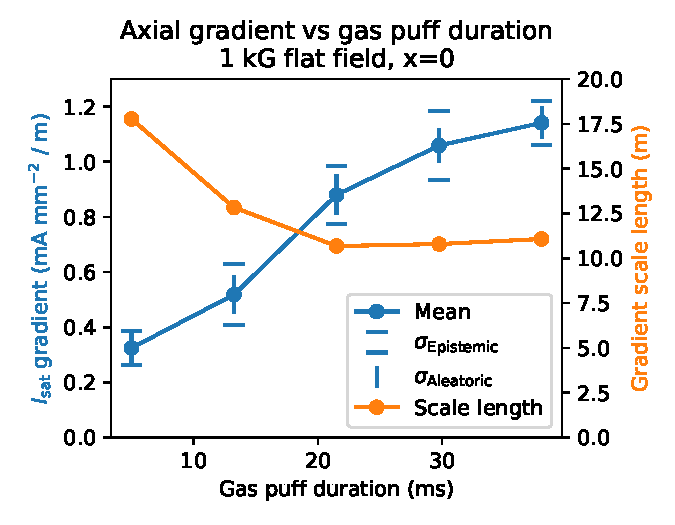
\includegraphics[width=\textwidth]{figures/axial-grad_gas-puff.pdf}
	\caption[size=12]{\label{fig:axial-grad_gas-puff.pdf}ML prediction: mean axial gradients decrease with decreased gas puff duration. Five durations are plotted between 5 and 38 ms (which are the bounds of the training data), evenly spaced. The gradient scale length also increases, indicating that the gradient change was not just from a decrease in the bulk $I_\text{sat}$.}
\end{figure}

\section{Optimizing profiles}
\label{sec:optimization}

%\begin{enumerate}
%	\item Table: machine settings predicted (done)
%	\item Measured vs predicted profiles (done)
%\end{enumerate}

One particular issue seen in LAPD plasmas is sharp axial density and temperature gradients. Some experiments require flat gradients, such as Alfv\'en wave propagation studies. We explore optimizing the axial $I_\text{sat}$ variation as an approximation to this problem. 
In addition, in this case the optimization problem is used as a tool to evaluate the quality of the learned model. This is a very demanding task because the trends inferred by the model along all inputs must simultaneously be accurate. Constraints on this optimization further increase the difficulty of the problem. Success in optimization provides strong evidence that the model has inferred relevant trends in predicting $I_\text{sat}$.
We quantify the flatness of the axial profile by taking the standard deviation of $I_\text{sat}$ of 11 points along the z-axis ($x,y=0$). The required LAPD state for attaining the flattest possible axial profile can be found by finding the minimum of this standard deviation with respect to the LAPD actuators (model inputs):
\begin{equation}
	\text{Inputs} = \operatorname*{arg\,min}_{\text{Inputs} \neq z} \operatorname*{sd}_{z}(I_\text{sat}|_{x=0})
\end{equation}
The largest axial variation can likewise be found by finding the maximum. The model inputs used for this optimization can be found in table \ref{tab:axial_optimization_inputs}. 

\begin{table}
	\small
	\centering
	\caption{Machine inputs and actuators for model inference}
	\label{tab:axial_optimization_inputs}
	\begin{tabular}{l l l l}
		Input or actuator & Range & Step & Count \\
		\hline
		Source field & 500 G to 2000 G & 250 G & 7 \\
		Mirror field & 250 G to 1500 G & 250 G & 6 \\
		Midplane field & 250 G to 1500 G & 250 G & 6 \\
		Gas puff voltage & 70 V to 90 V & 5 V & 5 \\
		Discharge voltage & 70 V to 150 V & 10 V & 9 \\
		Gas puff duration & 5 ms to 38 ms & 8.25 ms & 5\\
		Probe x positions & -50 cm to 50 cm & 2 cm & 51 \\
		Probe y positions & 0 cm & -- & -- \\
		Probe z positions & 640 cm to 1140 cm & 50 cm & 11 \\
		Probe angle & 0 rad & -- & --\\
		Run set flag & off and on & 1 & 2 \\
		Top gas puff flag & off and on & 1 & 2\\
		
	\end{tabular}
\end{table}

For this optimization we use an ensemble of five $\beta$-NLL-loss models with weight decay $\lambda=0$. The $\lambda=0$ model is used because it appears to give the most useful uncertainty estimate (seen fig. \ref{fig:extrapolation-profile-var_two}). The optimal machine actuator states are found by feeding a grid of inputs into the neural network. This variance estimate is not well-calibrated: the error of the predictions on the test set falls far outside the predicted uncertainty. However, this uncertainty can be used in a relative way: when the model is predicting far outside its training range, the predicted variance is much larger. The ranges of inputs into this model are seen in table. \ref{tab:axial_optimization_inputs}. These inputs yield 127,234,800 different machine states (times five models) which takes 151 seconds to process on an RTX 3090 ($\approx 4.2$ million forward passes per second) when implemented in a naive way. Note that gradient-based methods can be used for search because the network is differentiable everywhere but this network and parameter space is sufficiently small that a comprehensive search is tractable.

%This minimization disproportionately penalizes outliers. 
Like any optimization method, the results may be pathologically optimal. In this scenario, the unconstrained minimal axial variation is found when the $I_\text{sat}$ is only around 1 mA/mm$^2$, which is quite small and corresponds to $1\text{-}2\times 10^{12}$ cm$^{-3}$ depending on Te. The inputs corresponding to this optimum are in the second column of table \ref{tab:axial_optimization_results}. This density range is below what is required or useful for many studies in the LAPD. 

Since many physics studies require higher densities, we constrain the mean axial $I_\text{sat}$ value to be greater than 7.5 mA/mm$^{2}$ (roughly $0.5\text{-}2 \times 10^{13} \text{ cm}^{-3}$). The ``run set flag" is set to ``on" for cases to be validated (bolded in table \ref{tab:axial_optimization_results}) because we wish to keep the turbopumps on to represent typical LAPD operating conditions. In addition the ``top gas puff flag" was set to `off' to minimize the complexity of operating the fueling system on followup dataruns and experiments. Turning the top gas puff valve on is predicted to decrease the average $I_\text{sat}$ by $-2$ mA/mm$^2$ for strongly varying profiles, but otherwise the shapes are very similar.
The inputs corresponding to the maximum and minimum axial variation under these constraints can be seen in columns 3 and 4 of table \ref{tab:axial_optimization_results}. Out of curiosity we also consider what machine settings would lead to the greatest axial variation. The results of both of these optimizations can be seen in fig. \ref{fig:axial-var_prediction-vs-measurement}. The optimizations yield profiles that have the largest $I_\text{sat}$ values closest to the cathode, which is expected.

%As seen in fig. \ref{fig:best_axial_var}, the predicted uncertainty and test set RMSE are very large in comparison, which indicates the model may be far outside the bounds of the training data.

The predictions for the strongest, weakest, and intermediate axial variation cases is seen in fig. \ref{fig:axial-var_prediction-vs-measurement}. The intermediate case was chosen as somewhere around half way between the strongest and weakest case with a round index number (15000, in this case). The parameters for intermediate case are also enumerated in table \ref{tab:axial_optimization_results}. 

\begin{table*}
	\small
	\centering
	\caption{Machine inputs and actuators for optimized axial profiles}
	\label{tab:axial_optimization_results}
	\begin{tabular}{p{1.8 in} | p{0.75 in} p{0.75 in} p{0.75 in} p{0.8 in}}
		Input or actuator & Weakest & \textbf{Weakest} & \textbf{Strongest} & Intermediate \\
		$I_\text{sat}$ constraint (mA/mm$^2$) & $I_\text{sat} = $ any & $I_\text{sat}>7.5$ & $I_\text{sat}>7.5$ & $I_\text{sat}>7.5$\\
		\hline
		Source field      & 750 G   & 1000 G   & 500 G 	& 2000 G \\
		Mirror field      & 1000 G  & 750 G    & 500 G 	& 1250 G \\
		Midplane field    & 250 G   & 250 G    & 1500 G & 750 G \\
		Gas puff voltage  & 70 V    & 75 V     & 90 V 	& 90 V \\
		Discharge voltage & 130 V   & 150 V    & 150 V 	& 120 V \\
		Gas puff duration & 5 ms    & 5 ms     & 38 ms 	& 38 ms \\
		Run set flag      & on      & on       & on 	& on \\
		Top gas puff flag & on      & off      & off 	& off \\
	\end{tabular}
\end{table*}

The predicted configurations with the run set flag on and top gas puff flag off (bolded in table \ref{tab:axial_optimization_results} were then applied on the LAPD. The data collected, compared with the predictions can be seen in fig. \ref{fig:axial-var_prediction-vs-measurement}.

\begin{figure*}
	\centering
	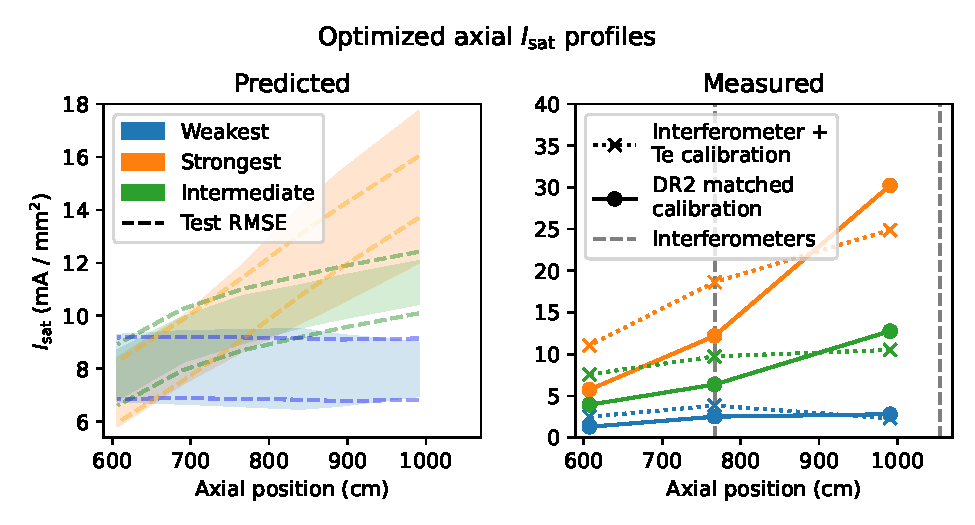
\includegraphics[width=360pt]{figures/axial-var_prediction-vs-measurement_paper.pdf}
	\caption[size=12]{\label{fig:axial-var_prediction-vs-measurement}Axial profiles, predicted and measured, for the optimized weakest (blue), intermediate (green), and strongest (orange) cases. a. The shaded region covers the mean prediction $\pm$ one standard deviation, and the dashed lines are $\pm$ the median cross-validation RMSE values. b. The measured $I_\text{sat}$ values are calibrated to \texttt{DR2} run 10 (solid lines), or using triple probe Te measurements on the probe and linearly extrapolating the interferometer measurements (dotted lines). The absolute values disagree between the predicted and measured values, but axial trends are consistent with the optimization.}
\end{figure*}

For the optimized axial profiles, the absolute value of the $I_\text{sat}$ predictions compared to measurement do not agree. All of the predicted profiles have overlapping predictions (within the predicted error) at the region furthest from the cathode, but the measured values do not show that behavior. Although the mean $I_\text{sat}$ value was constrained to be greater than 7.5 mA/mm$^2$, the measured mean was 2 mA/mm$^2$ for the weakest case. Despite these lack  of absolute 

The important thing here, however, is that the optimized LAPD settings, when implemented on the machine, do yield profiles with strong, intermediate, and weak axial variation. Although the minimum-$I_\text{sat}$ constraint was violated for the case of weakest axial variation case, this optimization would nonetheless be very useful for creating axial profiles of the desired shape. 

There are three contributing factors to the mismatch of the ML-predicted values and the real measured values. First, the condition of the cathode, such as its emissivity or temperature, in the plasma source region is unquantified and cannot be compensated for in data preprocessing or in the model itself. Second, the calibration of the Langmuir probes could differ substantially between runs. The probes in the training data run sets (\texttt{DR1} and \texttt{DR2}) were well-calibrated to each other within the run set, but were not absolutely calibrated. The probes used for verifying the optimization were not calibrated. A rough calibration was performed by linearly extrapolating interferometer measurements and using triple probes (dotted lines on the right panel in fig. \ref{fig:axial-var_prediction-vs-measurement}). A configuration identical to \texttt{DR2} run 10 was also measured to simultaneously correct cathode condition and probe calibration (solid lines on the right panel in fig. \ref{fig:axial-var_prediction-vs-measurement}). Langmuir probe calibration is discussed further in \ref{app:calib} Third, the original dataset may not have sufficient diversity to make accurate predictions on such a constrained optimization problem.

If this optimization were performed using the dataset instead of the model, the constrained search would encompass just 10084 shots out of the 131550 shots total in the training dataset, or around 7.7\%!. Including the on-axis constraint reduces the number of shots down to 303 (270 in the training set), or 0.23\% of all shots in the dataset. We conclude that this optimization of an arbitrary objective function, as done here, would be intractable using traditional, non-machine learning techniques because orders of magnitude more dataruns would need to be collected. 

Optimization requires correctly learning the trends of all inputs and how they interact. In addition, as seen from the shot statistics, the model was trained on very few shots in the constrained input and output space. These two factors -- the need for the model to learn all trends and the constrained search space -- combine to make an incredibly difficult task that functions as a benchmark for the model. These factors considered, it is not surprising that the model incorrectly predicts the absolute value. The uncertainty predicted by the model, though not well-calibrated, was nonetheless very large compared to the median test set RMSE, which indicates that the model was very uncertain. The model did get the trends correct, however; the optimized, measured profiles were strong, intermediate, or weak.

We did not check to see if the predicted optima were actually optima: an approximation of the local derivative using a finite-differenced technique would require much more run time on the LAPD than was available. 

\section{Discussion}
\label{sec:discussion}

%Feature engineering can be used to increase the performance of the linear model, such as adding a tanh feature for the x-profile, and can be continued to model the entire plasma. Symbolic regression or fitting to a function library may be ideal methods if simple profile prediction were the final goal. However, we are ultimately interested inferring trends in a much more complex input space, including time-varying signals and multiple diagnostics, where neural networks are more flexible and accurate. Symbolic methods are appealing because the fits are simple. However, even though a simple equation may fit the data well, it does not necessarily provide insight or relate to the underlying physics. In the context of this work, using a freeform fitting function like a neural network is more appropriate because it scales favorably with the number of examples and input size.

\subsection{Key achievements}

\todo{Expand discussion on uncertainty and why it's important}

To the authors' knowledge, this is the first time machine learning has been used to infer specific trends in magnetized plasmas and introduces the first open magnetized plasma dataset. Three examples of trend inference were shown in this paper: influence of magnetic geometry on plasma width, changes in the axial and radial profiles with changing discharge voltage, and the relationship of gas puff duration with axial gradient scale length. In addition, the axial profile was optimized by minimizing (or maximizing) the axial standard deviation. There is no other way of simultaneously uncovering many trends or finding optima without using an ML model over a diverse dataset. Traditionally, such studies would require extensive scans over grids to map the parameter space, but here it was accomplished with minimal data.

%A few examples of trend discovery and optimization were outlined in this paper, but there are many more trends and optimizations that can be evaluated using this model.  like the one described in this paper. An optimization could be performed using a gradient-based method, Bayesian optimization, or another optimization scheme, but the process would only be applicable to one specific optimization problem.

The trends inferred in this work, such as changing discharge voltages, gas puff durations, or mirror fields, would traditionally require a grid scan (varying one parameter at a time) in LAPD settings space. Here instead we are able to extract any trend covered by the training set with only a minimal amount of machine configurations sampled. Both data collection runs lacked absolute $I_\text{sat}$ calibration and had potential differences in cathode condition. Despite these issues the model learned trends that were exploited via optimization. 

Fundamentally, this model can predict $I_\text{sat}$ with uncertainty at any point in space covered by the training data. No other model exists that can perform this prediction. Traditionally this sort of capability would be possible only with a detailed and validated theoretical study. 

\subsection{Current limitations}

This study would be dramatically improved by collect more, diverse data. Only 44 of the 67 dataruns in this dataset were randomly sampled which is very small compared to the over 60,000 possible combinations in LAPD settings. In addition, there are many other LAPD settings that were not changed in this study, such as gas puff timings, gas puff valve asymmetries, wall/limiter biasing, cathode heater settings, operation of the north cathode, and so on. The bounds of the inputs were also conservative; all settings in this study could be pushed higher or lower with a small amount of risk to LAPD operations. In addition, the placement of the probes can be further varied and place outside the mirror cell, which would provide a more complete picture of LAPD plasmas and particularly axial effects.

Probe calibrations differed between the two training run sets (\texttt{DR1} and \texttt{DR2}), and a flag was introduced for the model to distinguish between them, but despite this deficiency combining the two run sets was advantageous for model performance. The condition of the cathode (e.g., electron emissivity and uniformity) also has a large impact on the measured $I_\text{sat}$. The improved model performance with the flag suggests that  inconsistencies between dataruns could be compensated for using latent variables if a generative modeling approach is to be taken. At the very least, this model provides a way to benchmark these differences in machine state.

On the model side, hyperparameter tuning can also be done. In this study we were not interested in squeezing out a few extra percent in MSE performance. Instead, we wanted to focus on the trends and insights that can be extracted from this model, rather than simple predictive accuracy. There may also be regimes in hyperparameter space where the uncertainty is better calibrated (perhaps using early stopping). Uncertainty estimation is important, even if the absolute uncertainty is not well-calibrated, because it can provide a useful relative estimate like what was shown in this paper. 

\subsection{Future directions}

The neural network architecture used here can readily scale to additional inputs and outputs; including time-series signals is the obvious next step. Integration of multiple diagnostics -- perhaps starting with individual models before combining them -- could enable inference of plasma parameters throughout the device volume. For example, combining triple probe electron temperature measurements with existing $I_\text{sat}$ data would allow density predictions anywhere in the plasma. This capability could enable in-situ diagnostic cross-calibration (e.g., the Thomson scattering density measurement) and prediction of higher-order distribution moments like particle flux. The model could be further enhanced by incorporating physics constraints such as boundary conditions (e.g., zero $I_\text{sat}$ at the machine wall) or symmetries. 

The problem presented here -- learning time-averaged $I_\text{sat}$ trends -- is fairly simple and required a relatively simple model. As demonstrated in this work, ML provides a way to explore regions of parameter space quickly and efficiently. Most physics studies on plasma devices (and fusion devices) are dedicated to a single particular problem, use grid scans, and are not useful to other experiments or campaigns. This work shows a way of using data and trends uncovered from other experimental studies. This work also demonstrates that random exploration can be a useful tool: the increased diversity of the aggregated data will always benefit an ML model whether or not the experiment discovers something new.

\section{Conclusion}
\label{sec:conclusion}

We demonstrate the first randomized experiments in a magnetized plasma experiment to train a neural network model. This learned model was then used to infer trends when changing field configuration, discharge voltage, or gas puff duration. This model was also used to optimize axial variation as measured by the standard deviation, which was validated in later experiments despite poor absolute error. 

We strongly advocate that all ML-based analyses in fusion should validate their models and gain insight by inferring trends, as demonstrated here. This validation step is crucial for ensuring that ML models capture physically meaningful relationships and the insights provided may provide direction for future research. We hope this is the first step towards automating fusion science.
%\pagebreak


\begin{figure}
%	\centering
	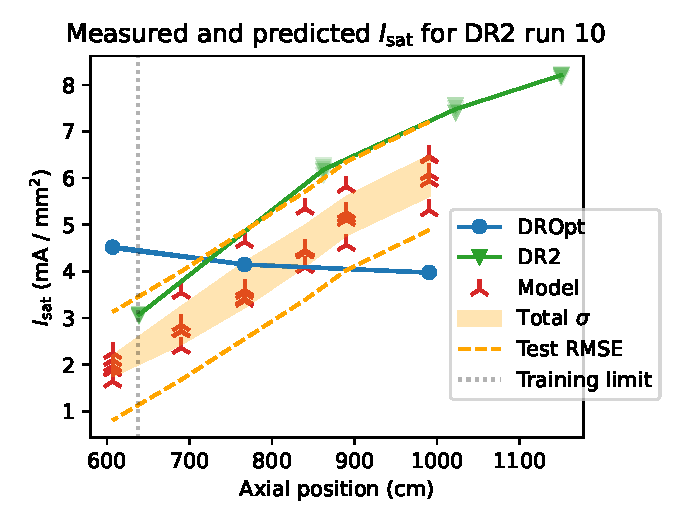
\includegraphics[width=\textwidth]{figures/DR2-10_LHS-30_valdiation.pdf}
	\caption[size=12]{\label{fig:DR2-10_LHS-30_valdiation}Comparison of original \texttt{DR2} profiles with the profiles from the optimization dataset (\texttt{DROpt}) for the same machine configuration. The $I_\text{sat}$ values in the \texttt{DROpt} dataset are not calibrated in this plot, indicating significant variation in probe calibration in this \texttt{DROpt} dataset.}
\end{figure}

\begin{figure}
%	\centering
	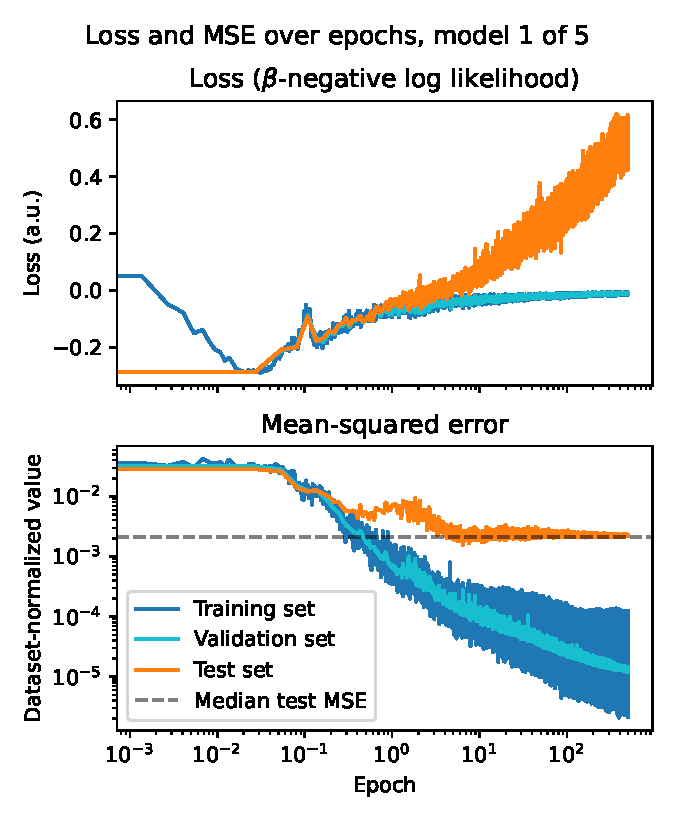
\includegraphics[width=\textwidth]{figures/beta-NLL_loss-mse.pdf}
	\caption[size=12]{\label{fig:beta-NLL_loss-mse}The loss and MSE for the training, validation, and test sets over the entire training duration of 500 epochs. The inclusion of the $\beta$ term in the loss function -- interpreted as a per-example learning rate -- makes the loss function no longer interpretable in simple terms. The mean-squared error benefits from longer training for all sets.}
\end{figure}

%\setcounter{section}{1} % reset numbering
%\appendix

\section{The open dataset and repository}
All the code to perform the ML portion of this study is available at this github repository: \texttt{https://github.com/physicistphil/lapd-isat-predict}. The training datasets are also available in that repository in the \texttt{datasets} directory. Additional data are available upon request. This is the first open dataset from a magnetized plasma device.

The plots used in this paper were made in jupyter notebooks, which are also uploaded. The final training code can be found in \texttt{train\_dense\_beta\_NLL.py}. Trained models are found in the \texttt{code/training\_runs} directory.

The history of many training runs can be found on Weights and Biases: \texttt{https://wandb.ai/phil/profile-predict} and the accompanying notes on these trained models are found in the associated pdf: \todo{upload pdf}.

\todo{Improve github readme and upload new stuff}

\section{Data bias \label{sec:app_bias}}
%\begin{enumerate}
%	\item x position distribution (done)
%	\item Table: breakdown by class (done)
%\end{enumerate}

\begin{figure*}
	\centering
	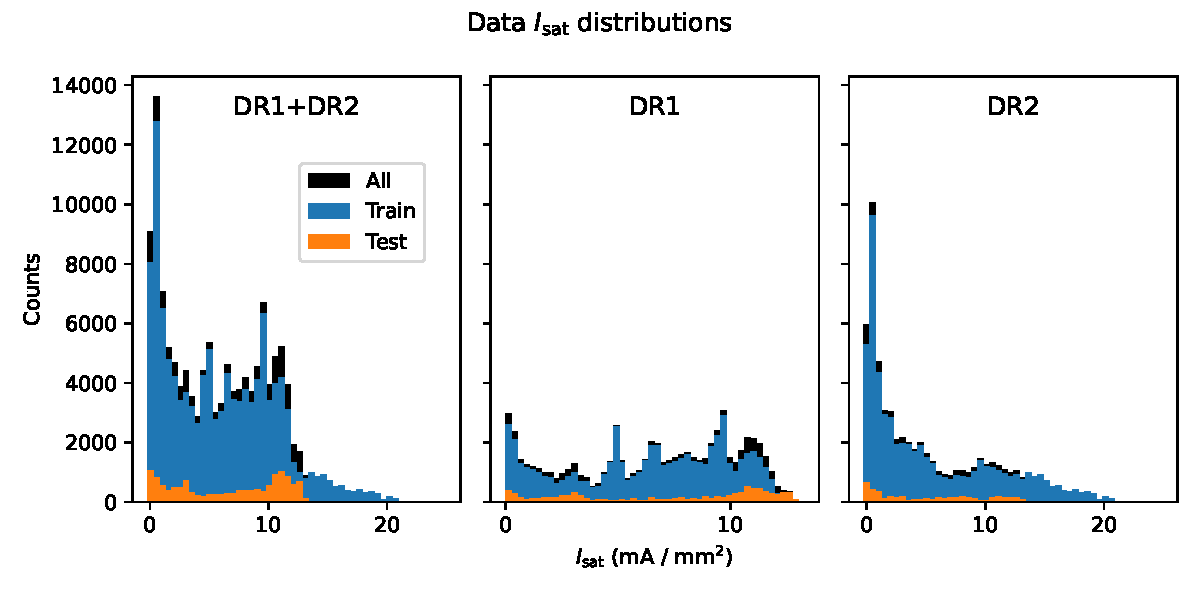
\includegraphics[width=\textwidth]{figures/PP1_02_isat_distribution.pdf}
	\caption[size=12]{\label{fig:PP1_02_isat_distribution}Distribution of $I_\text{sat}$ signals. \texttt{DR1} appears to have a more uniform distribution than \texttt{DR2} does. Combining the two datasets results in many $I_\text{sat}$ examples near 0 mA/mm$^2$ and a sharp decrease in number of examples above 10 mA/mm$^2$. From these histograms we expect or model to be biased towards fitting lower $I_\text{sat}$ values better, and to perform badly in cases with very high $I_\text{sat}$ values.}
\end{figure*}

Despite the best efforts to randomize the machine configuration, imbalance in the dataset will be present because of the relatively small amount of samples for the given actuator space. The distribution of $I_\text{sat}$ signals can be seen in fig. \ref{fig:PP1_02_isat_distribution}. The $I_\text{sat}$ distribution is clearly different for \texttt{DR1} and \texttt{DR2}, with \texttt{DR1} having a much flatter distribution. These distributions imply that if the model is constrained to sample from \texttt{DR2} via the run set flag, then the model is expected to predict a lower $I_\text{sat}$ value in general. When predicting from the model in general, performance will likely be worse for $I_\text{sat}$ values $\gtrsim 11$ mA/mm$^2$. 

\begin{table*}
\small
	\centering
	\caption{Data breakdown by class and dataset (percent)}
	\label{tab:data_frac}
	\begin{tabular}{lrrr|lrrr|lrrr}
		\multicolumn{4}{c|}{B source (G)} & \multicolumn{4}{c|}{B mirror (G)} & \multicolumn{4}{c}{B midplane (G)}\\
		\hline \hline
		& Train & Test & All && Train & Test & All && Train & Test & All \\
%		\cline{2-4} \cline{6-8} \cline{10-12}
		500 & 4.77 & 0 & 4.29 & 250 & 4.30 & 8.41 & 4.72 & 250 & 8.25 & 21.01 & 9.55 \\
		750 & 3.34 & 12.61 & 4.29 & 500 & 30.49 & 8.41 & 28.23 & 500 & 43.80 & 8.41 & 40.19 \\
		1000 & 43.13 & 78.99 & 46.78 & 750 & 6.68 & 16.81 & 7.72 & 750 & 6.62 & 52.19 & 11.27 \\
		1250 & 12.59 & 0 & 11.30 & 1000 & 28.85 & 57.97 & 31.82 & 1000 & 26.36 & 5.78 & 24.26 \\
		1500 & 19.23 & 0 & 17.27 & 1250 & 3.34 & 4.20 & 3.43 & 1250 & 9.24 & 0 & 8.30 \\
		1750 & 1.91 & 0 & 1.71 & 1500 & 26.34 & 4.20 & 24.08 & 1500 & 5.73 & 12.61 & 6.43 \\
		2000 & 15.03 & 8.41 & 14.35 & & & & & & & & \\
		\\
		\multicolumn{4}{c|}{Gas puff voltage (V)} & \multicolumn{4}{c|}{Discharge voltage (V)} & \multicolumn{4}{c}{Axial probe position (cm)} \\
		\hline \hline
		70 & 12.11 & 16.81 & 12.59  & 70 & 12.22 & 8.41 & 11.83    & 639 & 12.48 & 8.41 & 12.06 \\
		75 & 6.68 & 0 & 6.00     & 80 & 5.25 & 0 & 4.72      & 828 & 17.07 & 36.28 & 19.03 \\
		80 & 11.46 & 8.41 & 11.15   & 90 & 2.86 & 8.41 & 3.43      & 859 & 12.48 & 8.41 & 12.06  \\
		82 & 41.49 & 57.97 & 43.17  & 100 & 3.34 & 8.41 & 3.86     & 895 & 33.01 & 30.10 & 32.71 \\
		85 & 14.13 & 0 & 12.69   & 110 & 8.77 & 0 & 7.87     & 1017 & 12.48 & 8.41 & 12.06 \\
		90 & 14.13 & 16.81 & 14.40  & 112 & 20.62 & 0 & 18.52   & 1145 & 12.48 & 8.41 & 12.06 \\
                      & & & & 120 & 3.82 & 8.41 & 4.29     &                       & & & \\
                      & & & & 130 & 0.95 & 0 & 0.86     &                       & & & \\
                      & & & & 140 & 2.86 & 8.41 & 3.43     &                       & & & \\
                      & & & & 150 & 39.30 & 57.97 & 41.20  &                       & & & \\
		\\
		\multicolumn{4}{c|}{Gas puff duration (ms)} & \multicolumn{4}{c}{Vertical probe position (cm)}\\
		\cline{0-7} \cline{0-7}
		$38$ & 94.27 & 91.59 & 94.00 & $\approx 0$ & 36.26 & 46.08 & 37.26 & \\
		$<38$ & 5.73 & 8.41 & 6.00    & $\neq 0$ & 63.74 & 53.92 & 62.74    & \\
		\multicolumn{12}{l}{}
	\end{tabular}
\end{table*}


The distribution of the selected machine settings for all the dataruns is enumerated in table \ref{tab:data_frac}. Despite the randomization of the settings of 44 dataruns, the distribution is often uneven. This unevenness is exacerbated in the test set because that is a selection of 6 out of 67 dataruns. The remaining 23 non-random dataruns also contribute to the imbalance. For example, a source field of 1 kG and discharge voltage of 112 show up disproportionately in the dataset because data were collected at those settings while other equipment was being adjusted or calibrated.

Another source of imbalance is the vertical location of the probe: overnight dataruns are often planar so that machine time can be effectively used, so there are fewer planar dataruns but with many more shots, leading to more shots having a nonzero y-coordinate. This imbalance could have been avoided if the LAPD had programmable machine settings; this capability may be developed in the future.

\section{Data and training pipeline validation}

%\begin{enumerate}
%	\item Losses: overfitting and deep double descent (done)
%	\item Typical loss curve (done)
%\end{enumerate}

%A simple dense model (4 layers, 512 wide with one output; 794113 parameters, tanh activations) was trained. The model is also overfit on a single batch (128 examples) of training data to make sure that training progresses as expected. A deep double descent is observed as expected \cite{nakkiran_deep_2019,schaeffer_double_2023}. Training on a batch of 8 examples reaches $\approx$ 0 training loss after 50 steps. Plots of the train and validation losses can be seen in fig. \ref{fig:PP1_overfit_losses}. 

Multiple models were trained with varying depths and widths to verify that training loss decreases with increased model capacity. Doubling the layer width from 512 to 1024 moderately decreases the training loss; doubling the depth of the network from 4 to 8 layers has a larger impact. Increasing the width further to 2048 and depth to 12 layers has a dramatic impact on training loss, so this model and dataset are behaving nominally.

\todo{Discuss loss function, verifying no data leakage, and overfitting}

%\begin{figure}
%	\centering
%	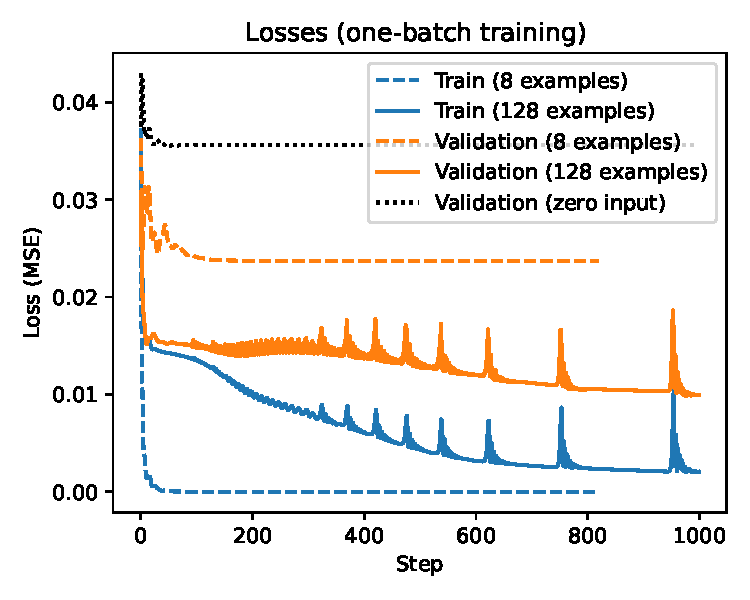
\includegraphics[width=\textwidth]{figures/PP1_overfit_losses.pdf}
%	\caption[size=12]{\label{fig:PP1_overfit_losses}Training and validation losses when overfitting the model. A deep double descent in the validation losses is observed when fitting a single batch of 128 examples. The 8-example batch hits near-zero loss after 50 steps. This process verifies our training process is functioning as expected. The spikes are from exploding gradients which can be mitigated by clipping the gradients. A model trained on blank data is also shown as the black dotted line.}
%\end{figure}

\section{Effect of $I_\text{sat}$ calibration \label{app:calib}}

%\begin{enumerate}
%	\item Interpolated $I_\text{sat}$ calibration vs DR2\_10 matchup (done)
%	\item Calibration 5 ms vs 38 ms gas puff (maybe not)
%\end{enumerate}

The Langmuir probes did not seem to be behaving correctly when the optimization validation data were taken. The probes showed an \emph{increasing} $I_\text{sat}$ profile when moving further from the cathode in the lowest gas puff condition, which is in direct disagreement with previous measurements and intuition. An example of this discrepancy can be seen in fig. \ref{fig:DR2-10_LHS-30_valdiation}, where a run from the original testing set (specifically \texttt{DR2} run 10) is duplicated. The probes for the validation run can be either corrected for by assuming the 5 ms gas puff run has a flat axial profile, or normalizing the probes to the \texttt{DR2} run 10 axial profile. Calibrating the probes using the \texttt{DR2} run 10 reference was the best way to go because it corrects for both probe discrepancies as well as changes in the condition (or emissivity) of the main cathode. 